\section{绘图(pgfplots)}\label{sec:plots}
\ifUsePgfplots
\begin{figure}[htbp]
\centering
\begin{subfigure}[t]{0.48\textwidth}
  \centering
  \begin{tikzpicture}
  \begin{semilogxaxis}[
    width=7cm,
    height=5cm,
    xlabel={$f$ (Hz)},
    ylabel={Magnitude (dB)},
    grid=both,
    legend style={font=\footnotesize,draw=none,at={(0.03,0.03)},anchor=south west}
  ]
  \addplot[blue,thick] coordinates {
    (10,-0.5) (50,-1.2) (100,-3) (300,-10) (1000,-22) (3000,-40) (10000,-60)
  };
  \addlegendentry{设计响应}
  \addplot[gray,dashed] coordinates {
    (10,-0.2) (50,-1) (100,-2.5) (300,-8) (1000,-18) (3000,-35) (10000,-55)
  };
  \addlegendentry{目标响应}
  \end{semilogxaxis}
  \end{tikzpicture}
  \caption{幅频响应}
\end{subfigure}
\hfill
\begin{subfigure}[t]{0.48\textwidth}
  \centering
  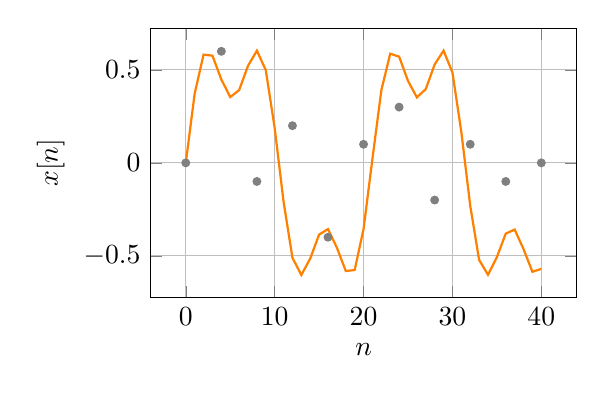
\begin{tikzpicture}
  \begin{axis}[
    width=7cm,
    height=5cm,
    xlabel={$n$},
    ylabel={$x[n]$},
    grid=major
  ]
  \addplot[orange,thick,domain=0:40,samples=41] {0.6*sin(deg(0.3*x)) + 0.25*sin(deg(0.9*x))};
  \addplot[black!50,mark=*,only marks,mark size=1.4pt] coordinates {
    (0,0) (4,0.6) (8,-0.1) (12,0.2) (16,-0.4) (20,0.1) (24,0.3) (28,-0.2) (32,0.1) (36,-0.1) (40,0)
  };
  \end{axis}
  \end{tikzpicture}
  \caption{时域样本}
\end{subfigure}
\caption{pgfplots 绘图示例}\label{fig:plot}
\end{figure}
\fi
